\documentclass[../Article_Sensitivity_Analsysis.tex]{subfiles}
\graphicspath{{\subfix{../Figures/}}}
\begin{document}
	
	\begin{comment}
		
	\label{CH: Results}
	
	To identify the global solution of Equations \ref{EQ:Formulation_1}, the optimization problem is solved multiple times, each starting from a random initial solution. Figure \ref{fig:scatter_T} compares the initial and final values of the cost function across multiple optimization runs. The shaded area spans from the smallest to the third smallest final values of the objective function. The black curves on the left and below the scatter plot represent the distributions of the initial and final cost function values, respectively. From Figure \ref{fig:scatter_T}, it can be observed that multiple local solutions exist for Case 1. The solution with the lowest cost function value is considered the global solution.
	
	\begin{figure}[h!]
		\centering
		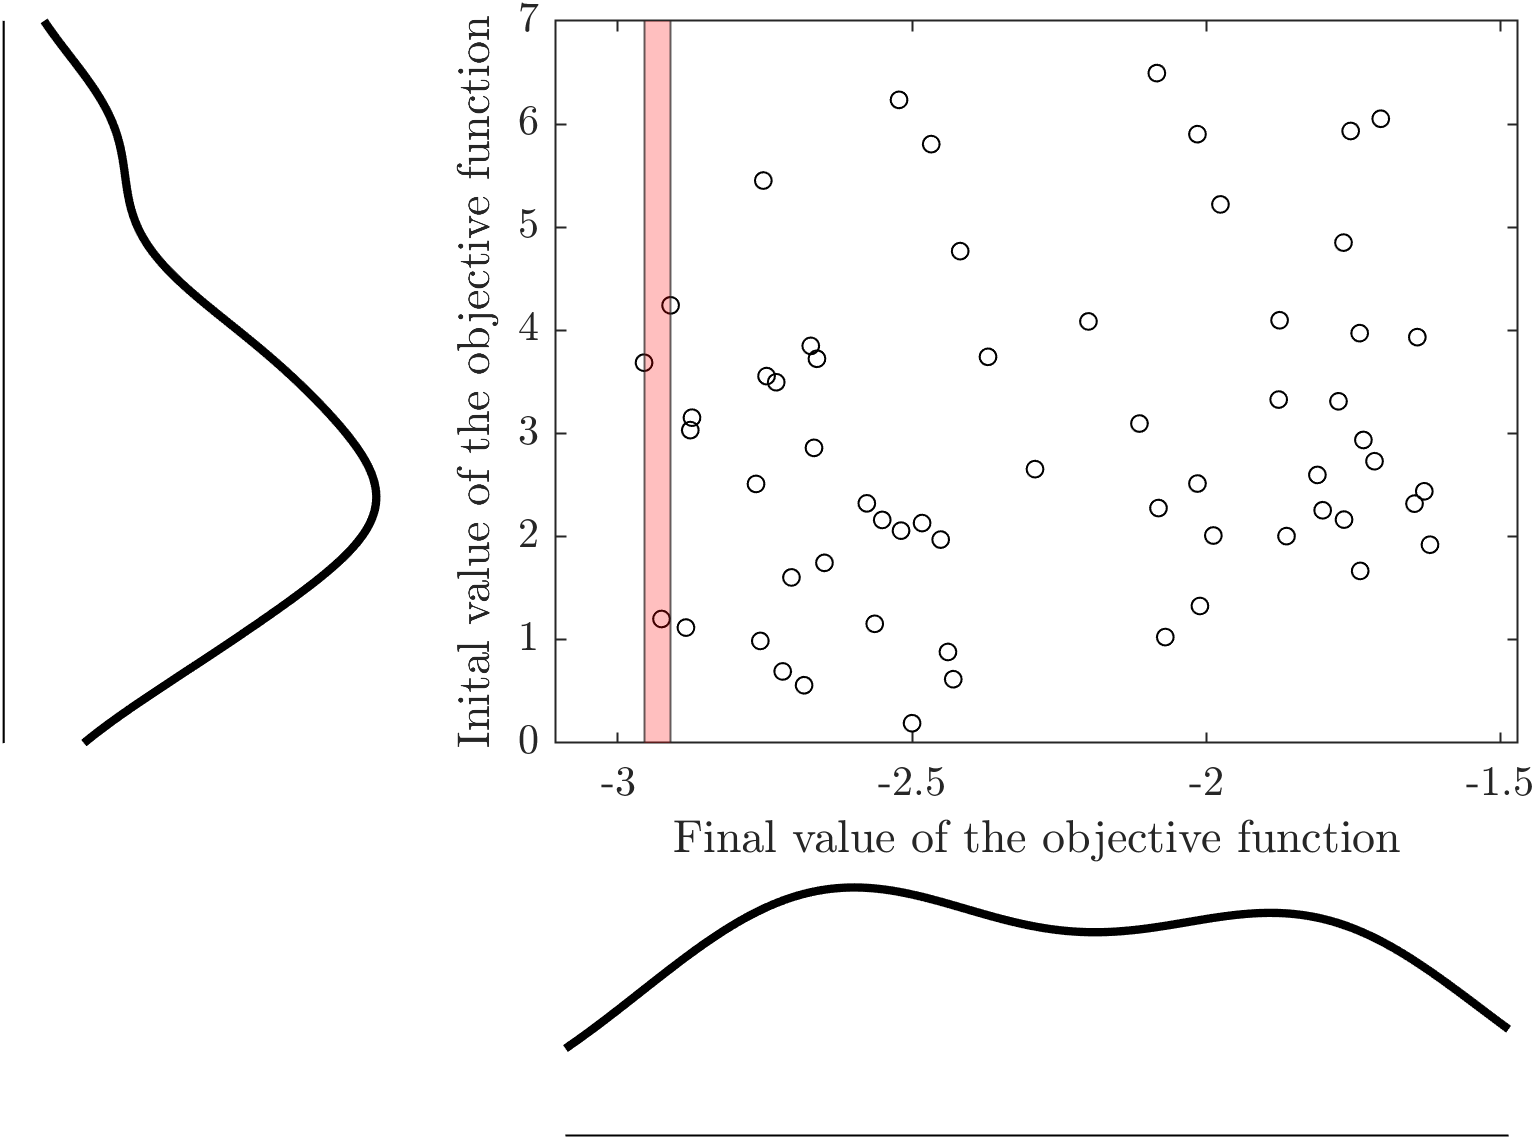
\includegraphics[width=\columnwidth]{Figures/Results/scatter_T.png}	
		\caption{Initial vs final values of the cost function}
		\label{fig:scatter_T}
	\end{figure}
	
	The optimal profiles of inlet temperature and mass flow rate are presented in Figure \ref{fig:profile_T}. One of the independent parameters in the analysed correlation is the mass flow rate, which is directly modified several times during the experiment. The second independent parameter is the Reynolds number, which can be affected by changes in the thermodynamic properties of the fluid. The thermal properties of CO$_2$ between $30^\circ$C and $40^\circ$C, assuming a constant pressure of 150 bar, vary only slightly. For instance, the dynamic viscosity changes from 67 to $80 \times 10^{-6}$ Pa$\cdot$s. The obtained profile of the inlet temperature shows minimal variation, suggesting a limited influence of inlet temperature on the extraction yield. Given the narrow operational window for inlet temperature at constant pressure, the mass flow rate becomes the primary variable to control.
	
	\begin{figure}[h!]
		\centering
		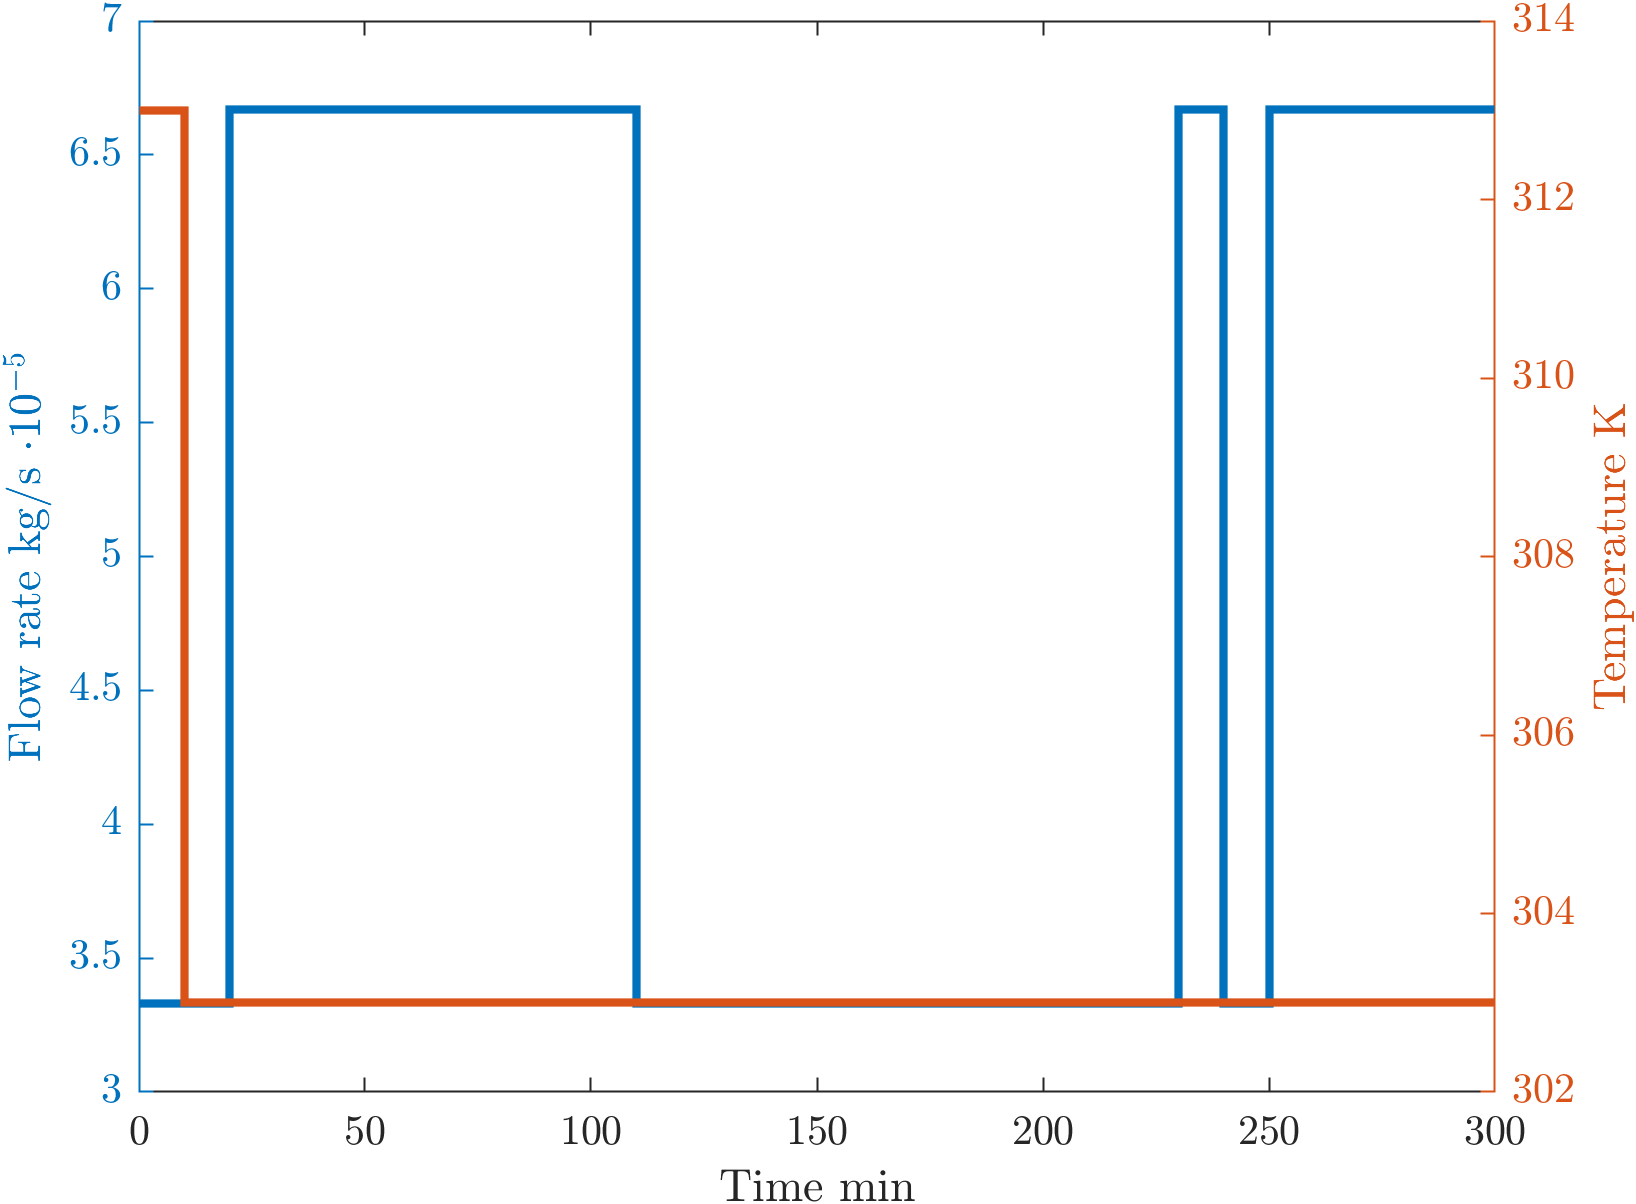
\includegraphics[width=\columnwidth]{Figures/Results/Profile_T_1.png}	
		\caption{Optimal temperature and mass flow rate profiles}
		\label{fig:profile_T}
	\end{figure}
	
	Similar to Case 1, Case 2 is solved multiple times starting from random initial solutions to identify the global solution. Figure \ref{fig:scatter_P} summarizes the changes in the objective function values across all optimization runs. It is evident that both the initial and final values of the cost function are significantly lower than any values obtained in Case 1. In Case 2, the wider operating range leads to more significant changes in the physical properties of CO$_2$ compared to Case 1. For example, the kinematic viscosity of CO$_2$ ranges from $48 \cdot 10^{-6}$ (at $40^\circ$C and 100 bar) to $90 \cdot 10^{-6}$ Pa$\cdot$s (at $30^\circ$C and 200 bar). The greater variability in pressure induces a more complex system response, including temperature variations, resulting in lower values of the objective function compared to Case 1.
	
	\begin{figure}[h!]
		\centering
		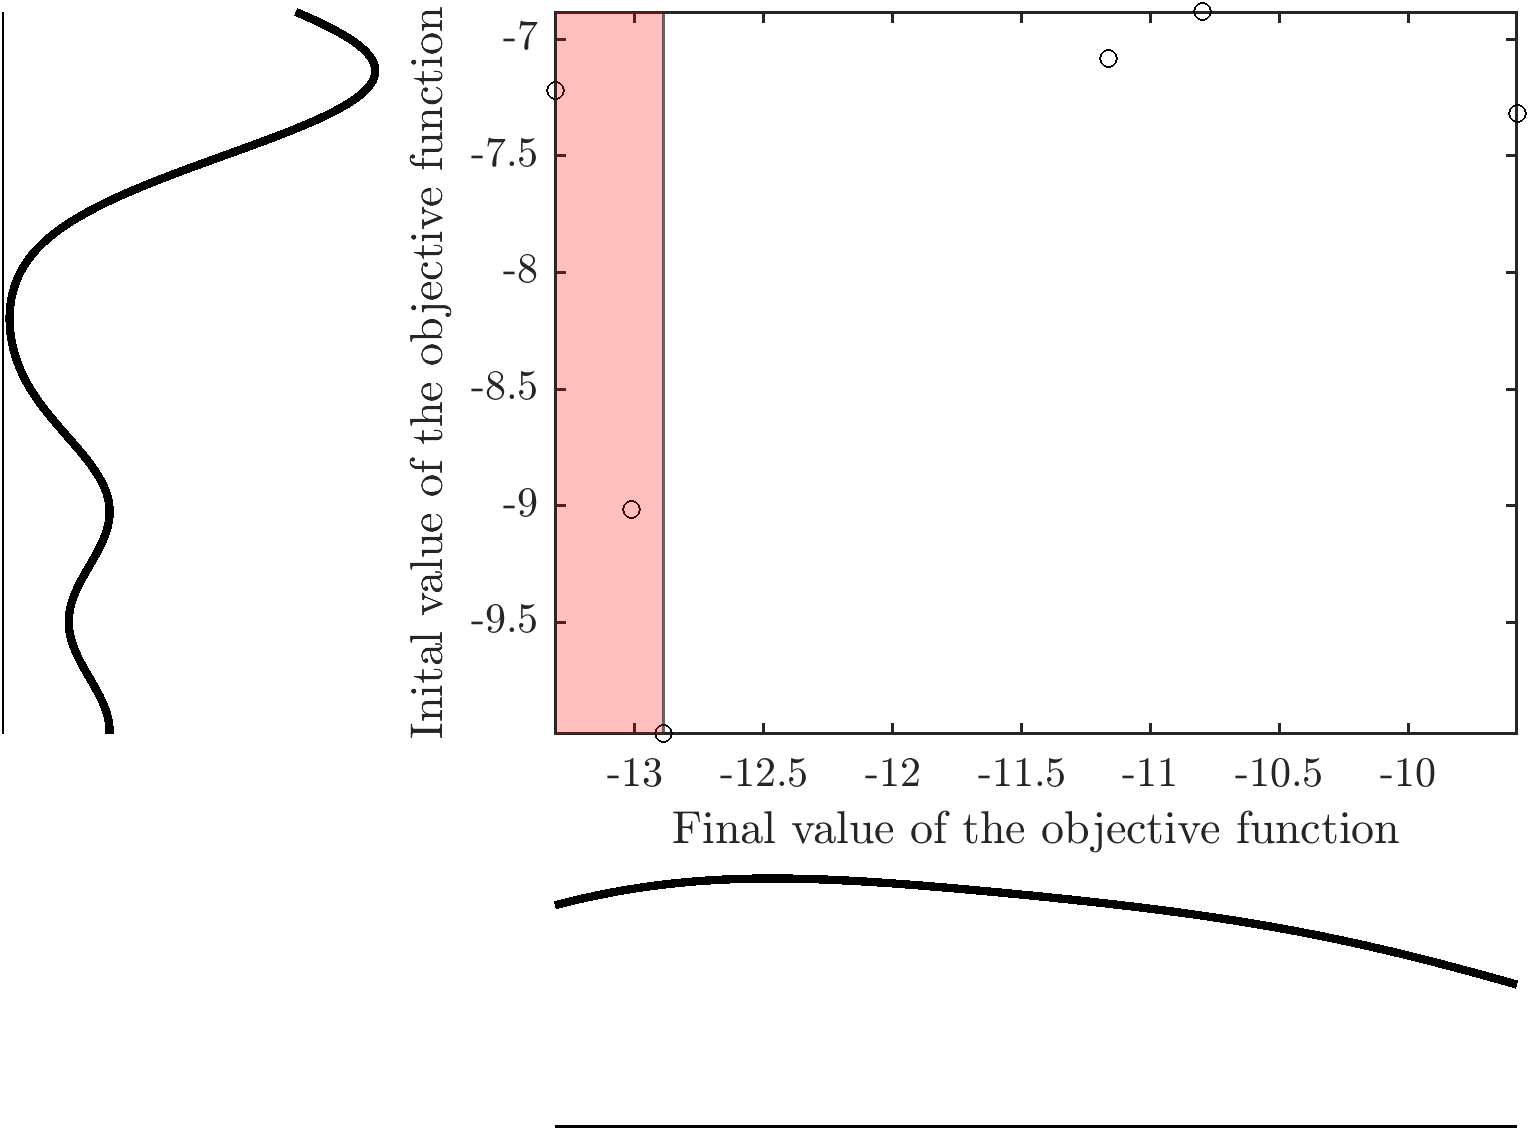
\includegraphics[width=\columnwidth]{Figures/Results/scatter_P.png}	
		\caption{Initial vs final values of the cost function}
		\label{fig:scatter_P}
	\end{figure}
	
	The optimal profiles of pressure and mass flow rate are presented on Figure \ref{fig:profile_P}. Similarly to case 1, only few changes in the mass flow rate are observed in the plot. In contrary to the inlet temperature, the pressure changes are frequently applied in the case 2. 
	
	\begin{figure}[h!]
		\centering
		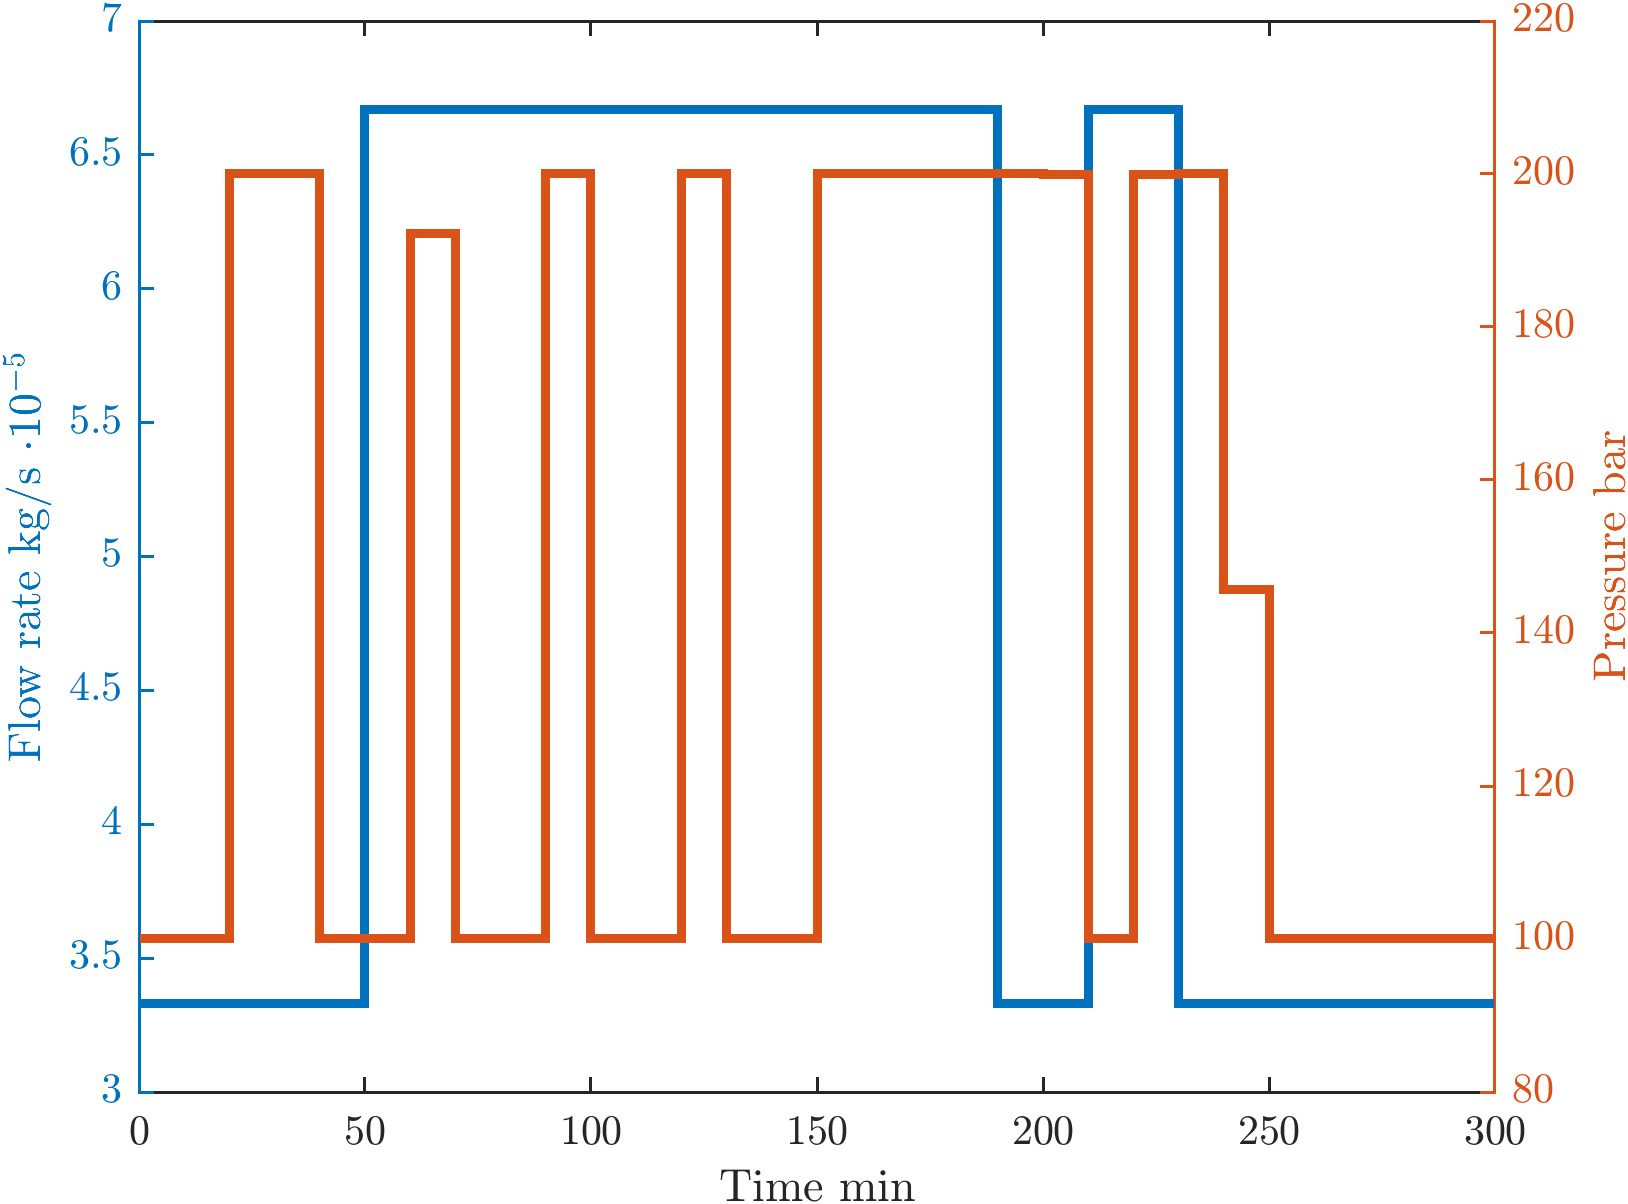
\includegraphics[width=\columnwidth]{Figures/Results/Profile_P_1.png}	
		\caption{Optimal pressure and mass flow rate profiles}
		\label{fig:profile_P}
	\end{figure}
	
	\end{comment}
	
	To identify the global solution for Equations \ref{EQ:Formulation_2}, the optimization problem is solved multiple times, each run starting from a random initial solution sampled from a uniform distribution. Figure \ref{fig:scatter} compares the initial and final cost function values across multiple optimization runs for all cases. The solution with the lowest cost function value is considered the global solution for each case.
	
	\begin{figure}[h!]
		\centering
		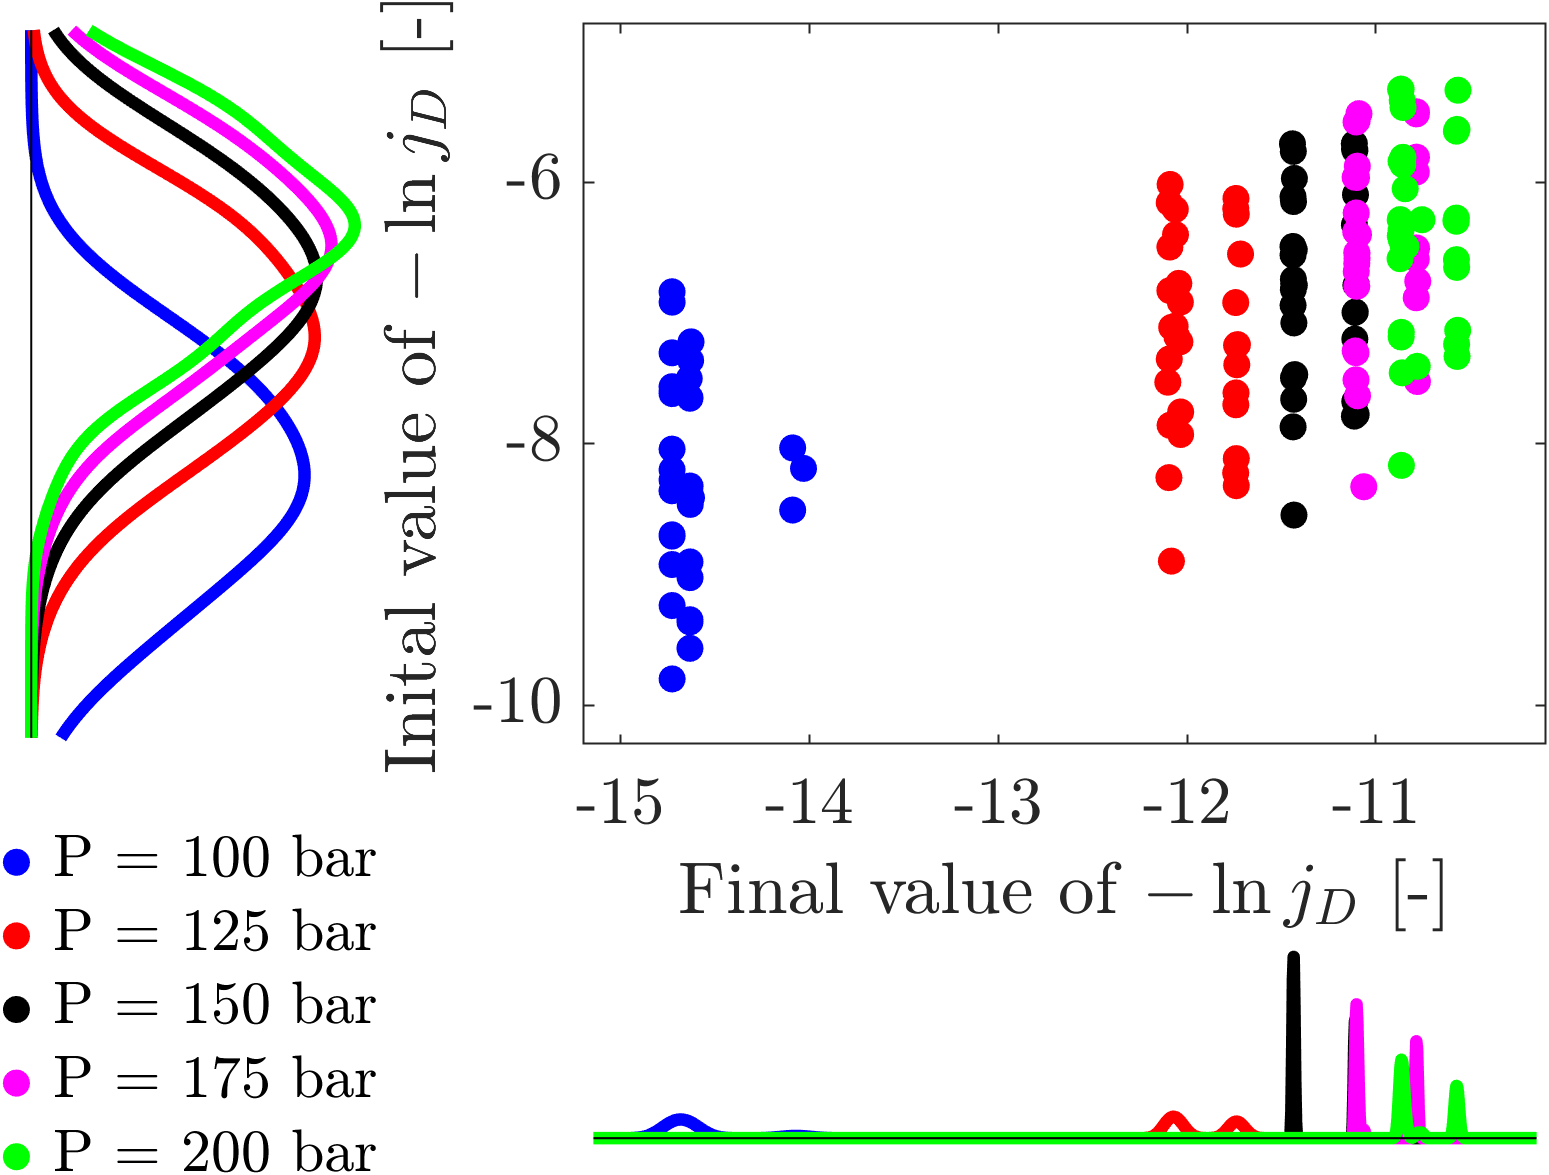
\includegraphics[width=\columnwidth]{Figures/Results/scatter.png}	
		\caption{Initial vs final values of the cost function}
		\label{fig:scatter}
	\end{figure}
	
	From Figure \ref{fig:scatter}, it is evident that multiple local solutions exist. By analyzing locations of the clusters in Figure \ref{fig:scatter}, it can be concluded that experiments conducted near the critical point provide more information regarding the correlation than those conducted farther from it. The closer the pressure is to the critical point, the larger the deviations in the physical properties of $CO_2$ caused by changes in the controls, leading to greater variation in the Reynolds number, and consequently to more informative experiments.
	
	For each pressure case, the profiles with the lowest value of the objective function are further analysed. As shown in Figure \ref{fig:profiles_T}, the dynamic behavior of the inlet temperature ($T^{in}$) for various cases in a supercritical CO2 extraction process. The initial temperature starts uniformly at $40~^\circ C$ for all cases but evolves differently depending on the operating conditions. These results underscore the sensitivity of supercritical CO$_2$ properties to control parameters such as temperature, particularly near the critical point. This observation aligns with the phenomenon that supercritical fluids exhibit properties like density and viscosity undergo strong non-linear changes around the critical point. At 200 bar the

	\begin{figure}[h!]
		\centering
		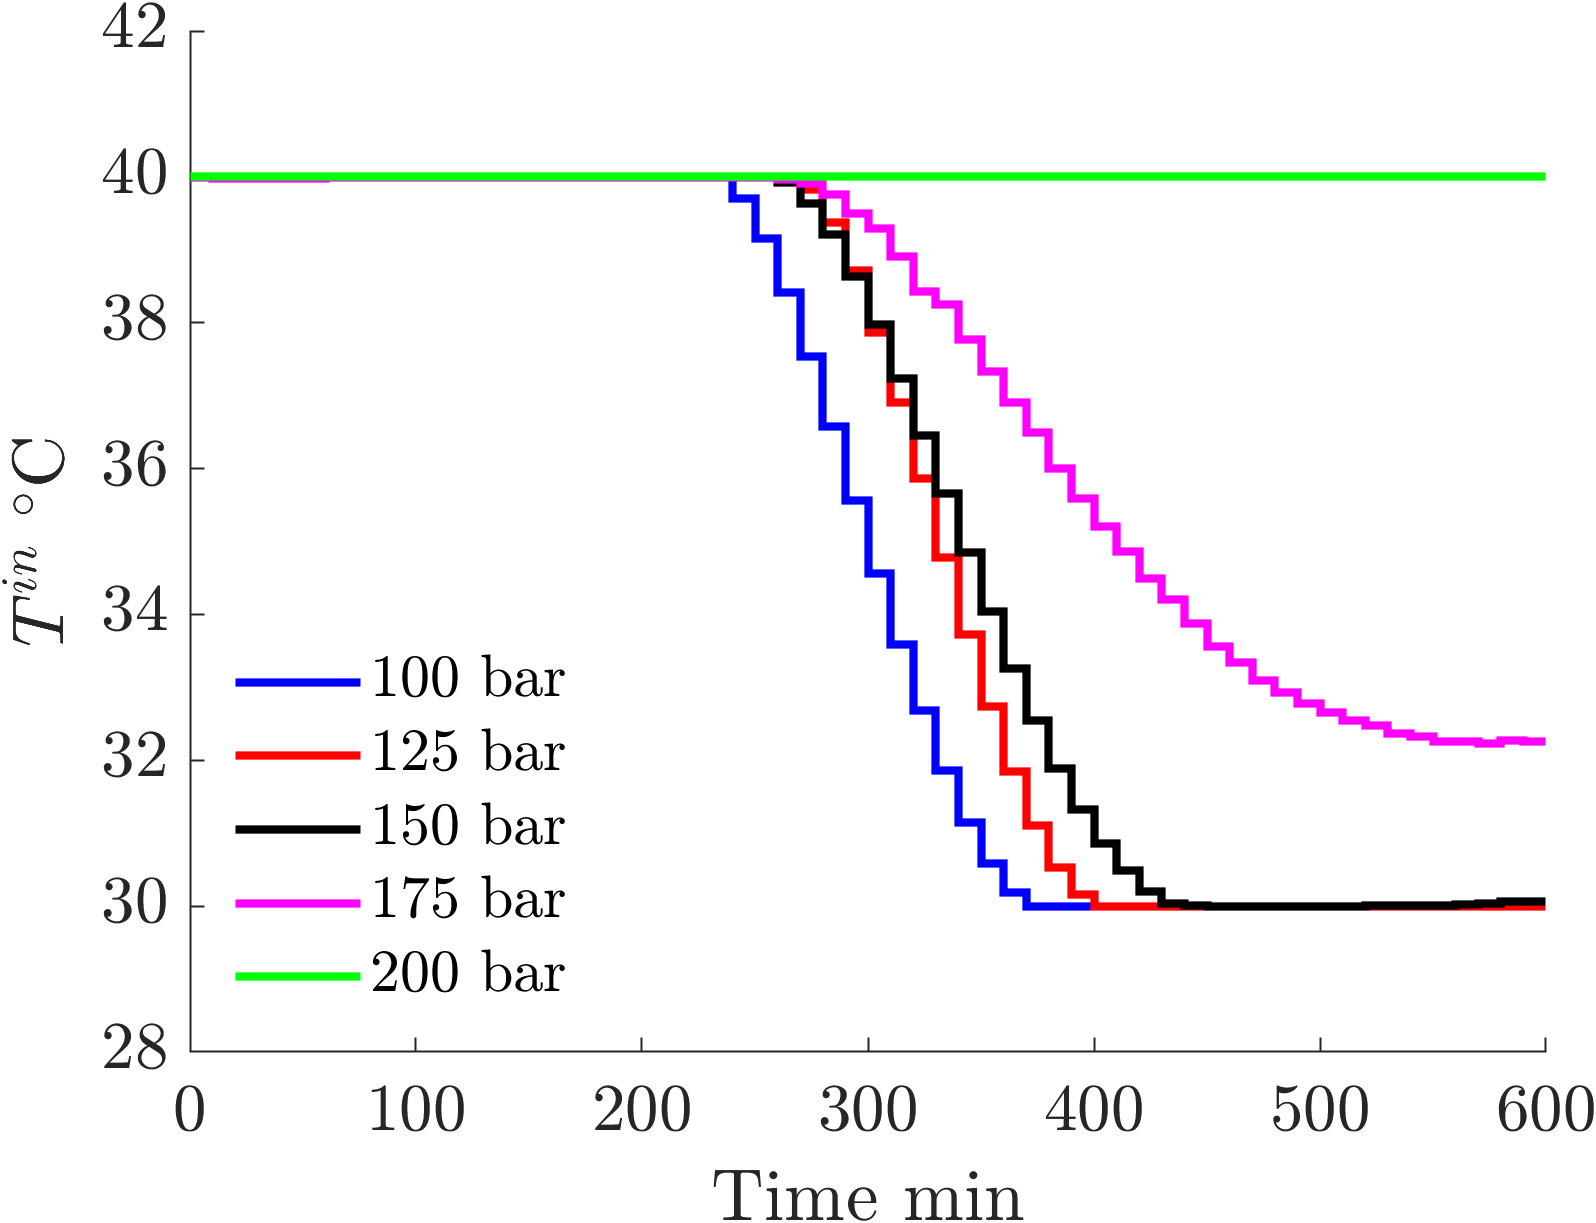
\includegraphics[width=\columnwidth]{Figures/Results/Profile_T.png}	
		\caption{Optimal inlet temperature profile}
		\label{fig:profiles_T}
	\end{figure}
	
	As presented in Figure \ref{fig:profiles_F}, in four out of five analysed cases, the corresponding mass flow rate profiles initially start at low values and gradually increase, reaching their maximum when the inlet temperature reaches its minimum. Later, the mass flow rates decrease to minimum values, and eventually, they rise again to reach their maximums at the final time. The only solution, which has different mass flow rate profile corresponds to pressure of 100 bar. The mass flow rate profile make the U-shape pattern, which starts the maximum value, then diminish to minimum and increases to the maximum value.
	
	\begin{figure}[h!]
		\centering
		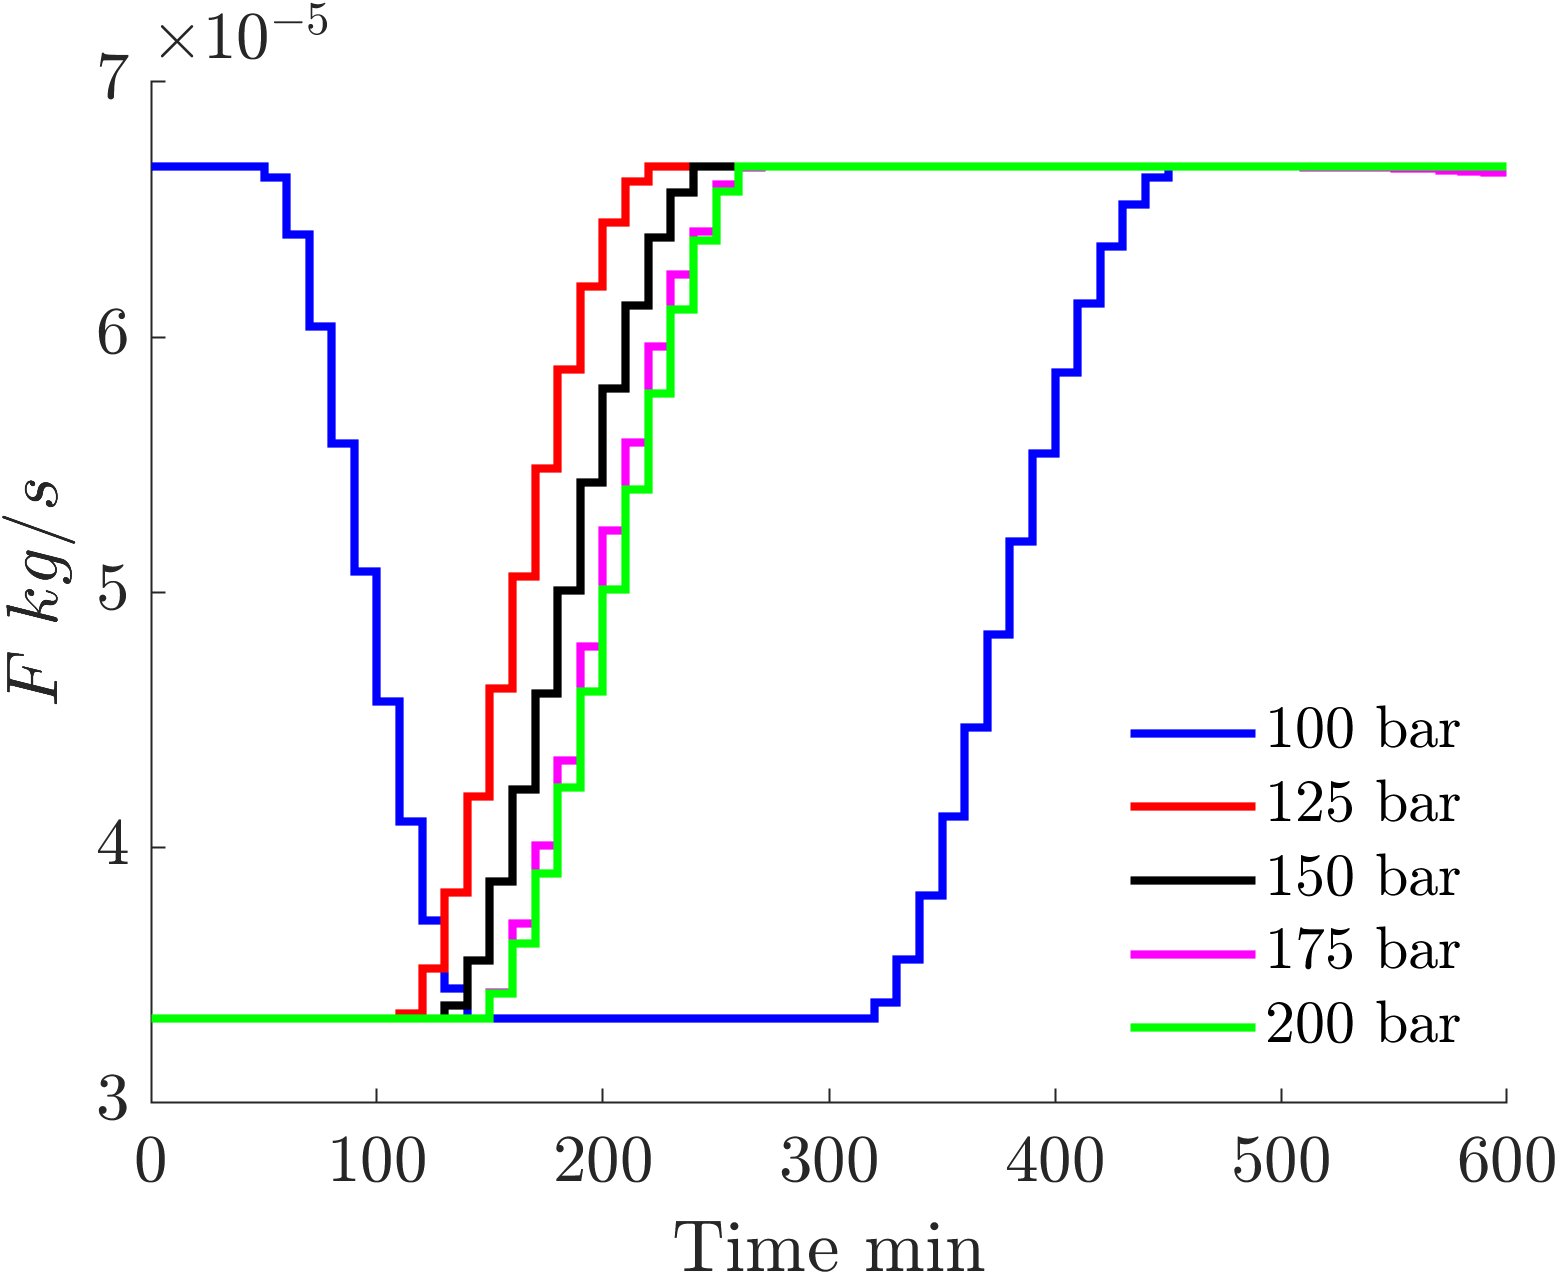
\includegraphics[width=\columnwidth]{Figures/Results/Profile_F.png}	
		\caption{Optimal mass flow rate profiles}
		\label{fig:profiles_F}
	\end{figure}
	
	Figure \ref{fig:profiles_y} shows the predicted yield curves. The yield and scatter plots show that the most informative experiments do not necessarily correspond to those with the highest yield. This is because the variation in $CO_2$'s physical properties differs depending on the system's pressure. At higher pressures, the extraction rates are high enough that the amount of collected oils becomes almost the same, which makes it difficult to distinguish between experiments. The optimal yield profiles are characterized by a wavy pattern rather than the smooth exponential-like pattern observed under steady conditions. This behaviour is expected, as the determinant of the Hessian matrix, when evaluated at a critical point of a function, is equal to the Gaussian curvature of the function considered as a manifold. When the sum of the Hessian determinants is maximized, the number of critical points increases, leading to the wavy pattern observed in the yield curves.
	
	\begin{figure}[h!]
		\centering
		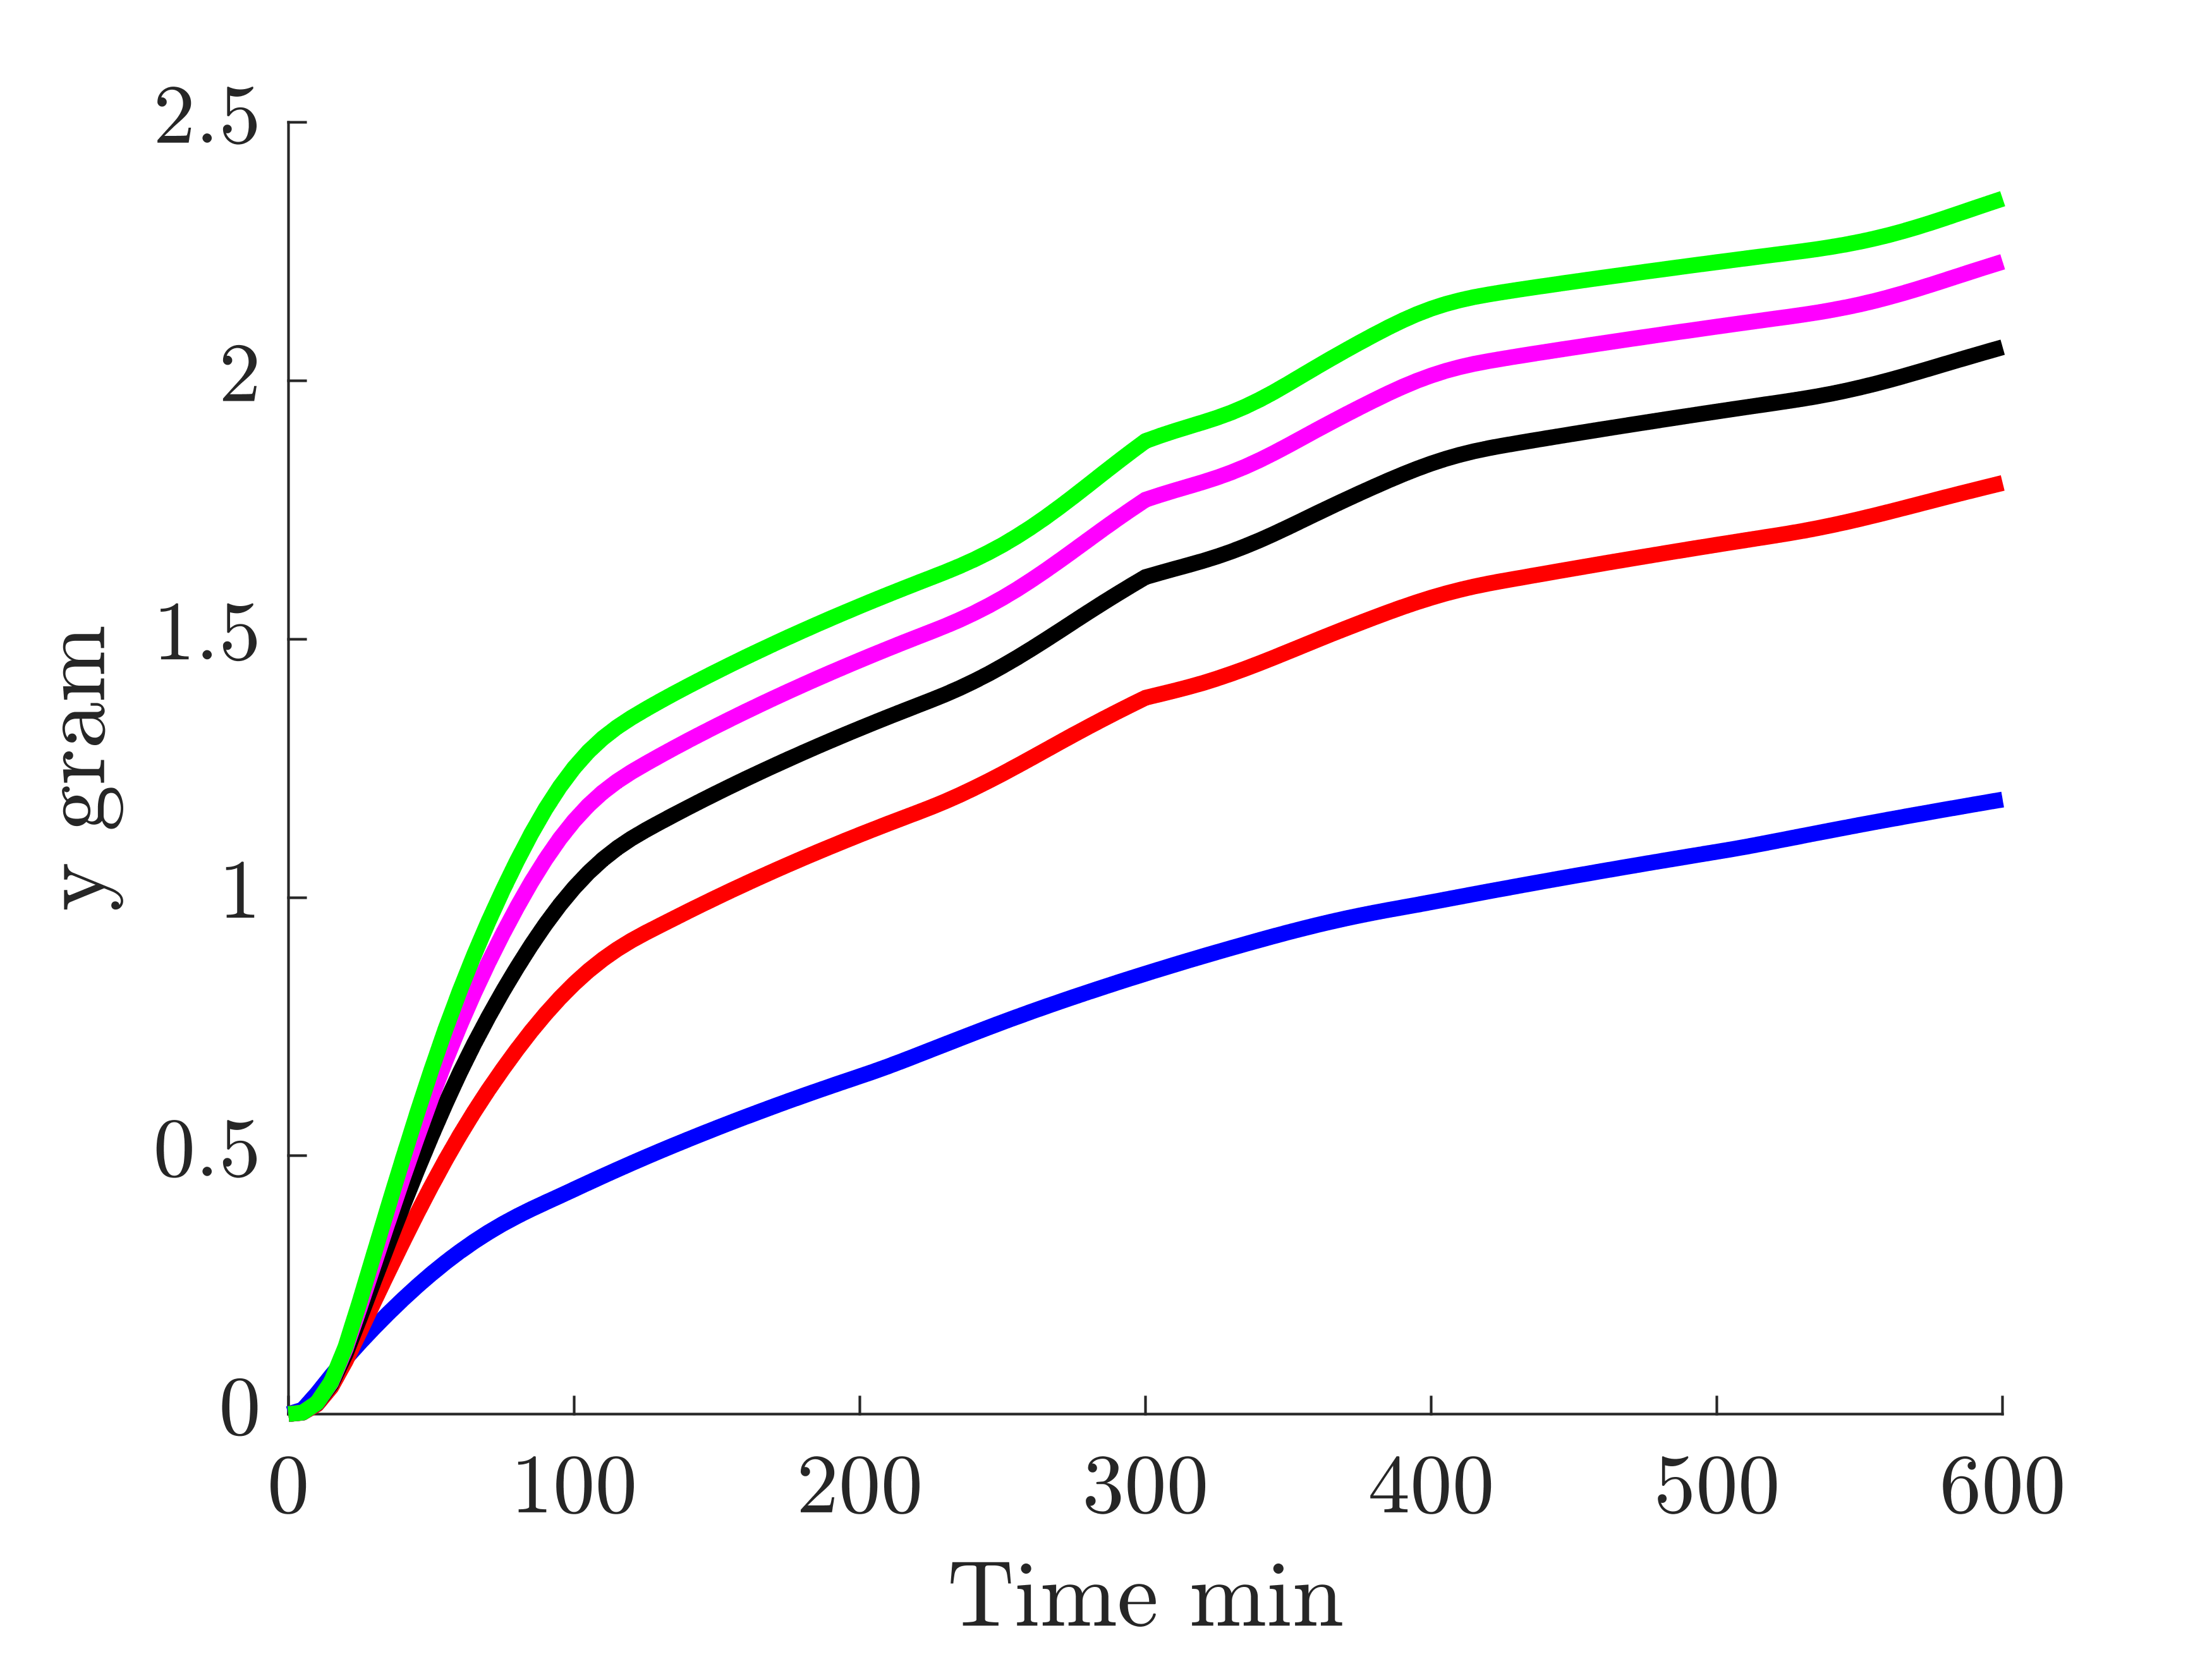
\includegraphics[width=\columnwidth]{Figures/Results/yield.png}	
		\caption{Optimal yield profiles}
		\label{fig:profiles_y}
	\end{figure}
	
\end{document}








































